\chapter{Method Overview}


\begin{figure}[b]
	\centering
	\includegraphics[width=\linewidth]{methodology/retrieval_pipeline.png}
	\caption{High level overview of the relocalization pipeline. Experimental data is split into a train and test set. Mapping, descriptor learning, and indexing is performed in an offline training stage. To localize a test query, we retrieve similar images from the database and perform feature matching and robust pose estimation.}
	\label{fig:pipeline}
\end{figure}

We perform relocalization in several steps, as shown in \fref{fig:pipeline}. First, to create an initial map of a scene, we perform visual odometry using DSO on each of a set of training videos. For each training sequence, this yields a set of per-frame camera poses and estimated semi-dense point clouds, plus an adjacency list of frames with co-observed points. We then extract features from each keyframe; rather than using an explicit feature detector, we simply evaluate the descriptor at every defined pixel in the semi-dense depth map. In a second pass, we merge multiple keyframe observations of the same point by computing the mean descriptor value, as in \cite{sattler2011fast} and \cite{schmidt2017self}.

In order to perform efficient retrieval of similar images, we compute an inverted index. We cluster features in the training set to create a visual word vocabulary and use the vocabulary to index training keyframes. We use the implementation of \cite{Sattler16CVPR}, which additionally filters results by their Hamming embeddings in order to remain discriminative while using a smaller visual vocabulary.

Finally, to relocalize, we compute descriptors for each frame in the test set, again at defined locations in the depth map. Note however that for the test set, we discard the depth information and do not compute the mean descriptor values, so that each test frame can be evaluated independently. Querying the inverted index now returns a list of plausible matches from the training set when given a query frame in the test set. We then compute a set of feature correspondences between each training and test frame, which thereby can be used with a RANSAC Perspective-n-Point solver to find the query pose (in the training sequence's frame of reference). We perform geometric verification, i.e.\ compute poses from the top 50 retrieved images, and return the one with the most inlier correspondences.

This chapter describes each of these aforementioned steps in detail.

\section{Visual Odometry}

We use DSO \cite{engel2017direct} as our method of choice to perform ``semi-dense'' visual odometry. DSO has a very particular frame representation, so we define some terminology for the sake of exactness.

\begin{figure}[h]
	\centering
	\includegraphics[width=\linewidth]{methodology/dso_pipeline.png}
	\caption{Flowchart of action performed in DSO. The system operates on two threads. The tracking thread performs coarse alignment of the most recent frame against the last keyframe, and also handles initialization. Meanwhile, the mapping thread curates a list of active keyframes, immature and active points, and active energy residuals, and performs Gauss-Newton optimization.}
	\label{fig:dso_pipeline}
\end{figure}

\subsection{Frame Representation}

DSO is a keyframe-based approach; not all frames are retained for the optimization process, and consequentially only frames designated as keyframes have meaningful semi-dense depth maps and high-accuracy bundle-adjusted poses. We denote the set of keyframe indices $\mathcal{F}$. In our experiments, when we perform visual odometry on the training set, we retain only the keyframes and discard everything else. Similarly, a practical approach to relocalization would be to run DSO on a testing sequence, and then only relocalize frames marked as keyframes. We do not do this (since subsampling the test set would muddle the comparison to prior work), but we observe that for a full end-to-end SLAM system, this would be a reasonable implementation.

During execution, DSO only optimizes parameters represented in the current window of active keyframes. When the number of tracked keyframes exceeds a threshold (7 by default), or when the quality of a keyframe is poor, it is marginalized out of the energy function and deleted. Notably though, keyframes are not necessarily removed in FIFO order, so a few high quality keyframes earlier in a sequence may serve to stabilize the estimated trajectory. After removal, DSO makes no attempt to relocalize against marginalized frames or to perform large-scale global loop closure. For this reason, it belongs to the realm of visual odometry algorithms, and can suffer from drift over time.

DSO is direct, in that it does not explicitly track the world as a set of 3D points. Rather, each point is associated with a host frame, and is defined by its inverse depth and the host frame's camera pose. Specifically, suppose keyframe $i \in \mathcal{F}$ has a set of pixels $\mathcal{P}_i$ for which the inverse depth is defined. For a pixel $\boldsymbol{p} \in \mathcal{P}_i$, we can define its world position $X_{\boldsymbol{p}} \in\mathbb{R}^3$ as a function of the inverse depth $d_{\boldsymbol{p}} \in \mathbb{R}^+$ and the camera-to-world transformation $(\boldsymbol{R}_i, \boldsymbol{t}_i)$:

\begin{equation}
X_p = \boldsymbol{R}_i \Pi^{-1}(\boldsymbol{p}, d_{\boldsymbol{p}}) + \boldsymbol{t}_i
\end{equation}

This is a purported advantage of DSO, since each additional tracked point adds only one unknown parameter ($d_{\boldsymbol{p}}$) instead of three. Here, $\Pi$ represents the camera intrinsic parameters and projection operation, and likewise $\Pi^{-1}$ represents a back-projection. For example, given a coordinate $X$ in the local coordinate frame, for a pinhole camera model oriented along the $z$-axis, $\Pi$ performs multiplication by a pinhole calibration matrix followed by a nonlinear projection:

\begin{equation}
\Pi(X) = 
\begin{bmatrix}
\frac{X'_0}{X'_2} \\
\frac{X'_1}{X'_2}
\end{bmatrix}
\text{, where } X' = KX =
\begin{bmatrix}
f_x & 0 & c_x \\
0 & f_y & c_y \\
0 & 0 & 1
\end{bmatrix} X
\end{equation}

And $\Pi^{-1}$ performs the opposite, assuming the depth is given for the pixel $\boldsymbol{p} = (p_1, p_2)$:

\begin{equation}
\Pi^{-1}(\boldsymbol{p}, d_{\boldsymbol{p}}) = 
K^{-1}
\begin{bmatrix}
p_1 \\
p_2 \\
1
\end{bmatrix}
\frac{1}{d_{\boldsymbol{p}}}
=
\begin{bmatrix}
\frac{1}{f_x} & 0 & -\frac{c_x}{f_x} \\
0 & \frac{1}{f_y} & -\frac{c_y}{f_y} \\
0 & 0 & 1
\end{bmatrix} 
\begin{bmatrix}
p_1 \\
p_2 \\
1
\end{bmatrix}
\frac{1}{d_{\boldsymbol{p}}}
\end{equation}

Note that here $d_{\boldsymbol{p}}$ is the \textit{inverse} depth, so for a point with local coordinates $(x, y, z)$, its inverse depth is the reciprocal $d = \frac{1}{z}$. This used rather than the depth because it is assumed that the inverse depth itself is Gaussian-distributed (and therefore the depth itself has a longer-tailed distribution).

In addition, for every point $\boldsymbol{p}$ in a host frame, DSO maintains a list, $\text{obs}(\boldsymbol{p})$, of frames which mutually observe the point. As a result, we can re-project points hosted by one camera $i$ into a second with index $j\in \text{obs}(\boldsymbol{p})$ (and vice versa) to get an even more dense depth map (assuming the points lie within the image bounds).

\begin{equation}
\boldsymbol{p}' = \Pi(\boldsymbol{R}_j^T (\boldsymbol{R}_i \Pi^{-1}(\boldsymbol{p}, d_{\boldsymbol{p}}) + \boldsymbol{t}_i - \boldsymbol{t}_j))
\end{equation}

Here $\boldsymbol{p}'$ is the new coordinate in frame $j$. This can even be done between a keyframe and a non-keyframe, albeit with less accuracy since non-keyframes have only a coarsely estimated pose. When we consider semi-dense depth maps later in this document, we assume that this re-projection step has been performed. In some cases, multiple points may re-project onto the same pixel in a frame; in that scenario, we simply keep the first point encountered.

\begin{figure}[h]
	\centering
	\includegraphics[width=0.5\linewidth]{methodology/depth_map.png}
	\caption{Example of a semi-dense inverse depth map from one scene. Depth estimates are largely distributed along edges, and absent in areas with little texture, like walls. On highly-textured areas, like the carpet, points are distributed more evenly.}
	\label{fig:depth_map]}
\end{figure}

Finally, we note that each DSO keyframe actually manages two classes of points in its depth map. Initially, every chosen point is designated as an ``immature'' point, and its depth is estimated by filtering it with observations in succeeding frames. This operates in the same manner as \cite{engel2013semi}, in which multiple observations of Gaussian-distributed inverse depths are combined. For these points, $\text{obs}(\boldsymbol{p})$ is not used, assumedly due to the high uncertainty and high likelihood of accruing outliers. Once we are sufficiently certain of a point's inverse depth, it graduates to being an ``active'' point, and residuals are computed by projecting it into all active keyframes, which initializes the set $\text{obs}(\boldsymbol{p})$. From here, the residual persists until the host frame is removed from the optimization, the point goes out-of-bounds, or it is otherwise classified as an outlier.

It generally takes several frames before an immature point is activated, and most points in the depth map are never activated. We discard immature points in this work, as they have high variance in their depth estimation, and their depth is not necessarily consistent with all keyframes in the active window. We anticipate that for future work, these could be incorporated into the final pose estimation using dense bundle adjustment, as in \cite{engel2014lsd}.

So far, we have described the data representation used in DSO, but not actually how pixels are selected, or how the optimization is performed. The core operation of DSO is easiest to understand by following the life of a frame, as detailed in \fref{fig:dso_pipeline}. In its implementation, DSO is split into a high-priority tracking thread, and a mapping thread which can tolerate some delay in processing. Regardless though, a frame starts by being added to the tracking thread, and it is propagated to the mapping thread, where it is either discarded or retained and kept as a keyframe for tracking.

\subsection{Pixel Selection}

Pixel selection is performed while initializing the very first frame, and also at the very end of the mapping loop for subsequent keyframes. To select pixels for depth tracking, DSO uses a two step system, in which they first filter pixels by a local threshold, and then adaptively select points until a reaching a sufficient density. We give a high level overview, omitting some details about image pyramid construction and gradient smoothing.

To filter pixels, the method first computes the magnitude of gradient $|\nabla I[r, c]|$ for every row $r$ and column $c$ in the image; the gradient is computed via central differences. The method then divides the image into blocks of size $32 \times 32$ and computes the median $\bar{g}$ in each block. Pixels are subsequently considered only if their absolute gradient is greater than $\bar{g} + g_\text{th}$, with $g_\text{th} = 7$ by default. In this regard, we are filtering out all but an upper quantile of pixel gradients. Next, DSO divides the image into another set of blocks, this time with size $d \times d$. $d$ is computed adaptively, but is generally around $3$. The maximal gradient pixel in each $d \times d$ block is selected, so that in the end, the fraction of image pixels selected is at most $\frac{1}{2 d^2}$. For small integer values of $d$, this is on the order of the full image resolution, hence the ``semi-dense'' designation. These points may be further subsampled if a smaller density is desired (by default, DSO subsamples this to between 600-1500 points, though we use values in the high thousands for this thesis).

%\begin{algorithm}
%	\caption{DSO Pixel Selection}\label{alg:pixel_select}
%	\hspace*{\algorithmicindent} \textbf{Input} An image $I$ with dimensions $W \times H$, threshold $g_{\text{th}}$\\
%	\hspace*{\algorithmicindent} \textbf{Output} A 2D boolean array
%	\begin{algorithmic}[1]
%		\Procedure{select}{}
%		
%		\State let $G$ be a $W \times H$ array
%		\For{$r \in \{1 \ldots H\}$, $c \in \{1 \ldots W\}$}
%			\State $G[r,c] \gets |\nabla I[r,c]|$ 
%			\Comment{Compute $\nabla$ as central differences}
%		\EndFor
%		
%		\State Divide $I$ into $32 \times 32$ blocks
%		\State let $T$ be a $W \times H$ array
%		\let $M$ by a 
%		\For{each block with endpoints $b = (r_1, r_2, c_1, c_2)$}
%			\State Compute $\bar{g}$ as the median of $G[r, c], r\in\{r_1 \ldots r_2\}, c \in \{c_1 \ldots c_2\}$
%	\end{algorithmic}
%\end{algorithm}

\subsection{Optimization}

After sufficiently many pixels have been selected and we have bootstrapped an initial depth estimate of several frames, we can perform bundle adjustment of our estimate. We reproduce the full DSO energy term here for clarity, but refer readers to \cite{engel2017direct} for a proper analysis. The energy minimized by DSO is the following energy:

\begin{equation}
E_{\text{photo}} = \sum_{i \in \mathcal{F}} \sum_{\boldsymbol{p} \in \mathcal{P}_i} \sum_{j \in \text{obs}(\boldsymbol{p})} E_{\boldsymbol{p}ij}
\end{equation}

Where $E_{\boldsymbol{p}ij}$ is the photometric error in the reprojection:

\begin{equation}
E_{\boldsymbol{p}ij} = \sum_{\boldsymbol{q} \in \mathcal{N}_{\boldsymbol{p}}} w_{\boldsymbol{p}} \rho_\gamma((I_j[\boldsymbol{p}'] - b_j) - \frac{e^{a_j}}{e^{a_i}}(I_i[\boldsymbol{p}] - b_i))
\end{equation}

Here $\mathcal{N}_{\boldsymbol{p}}$ represents a small window of neighboring points (the authors suggest a checkerboard pattern of neighboring points), $\rho_\gamma$ represents the Huber norm, $\boldsymbol{q}'$ denotes the reprojection of $\boldsymbol{q}$ as seen earlier, and the terms $a_i$, $b_i$, $a_j$, $b_j$ represent an affine transformation of lighting conditions from frame to frame due to changing exposure values. The weight $w_{\boldsymbol{p}}$ is a weighting term on the gradient, with

\begin{equation}
w_{\boldsymbol{p}}  = \frac{c^2}{c^2 + ||\nabla I_i(\boldsymbol{p})||_2^2}
\end{equation}

The full state of the system is then the geometric parameters $(\boldsymbol{R}_i, \boldsymbol{t}_i)$ and $d_{\boldsymbol{p}}$ for $\boldsymbol{p} \in \mathcal{P}_i$ and the photometric calibration parameters $(a_i, b_i)$ over all keyframes $i \in \mathcal{F}$.

\subsection{Initialization and Coarse Tracking}

The above energy is minimized for keyframes, but how is tracking performed for non-keyframes, and is the system initialized?

For coarse tracking of all new frames, DSO seeks to minimize a slightly different energy. The authors project all active residuals to the most recently tracked keyframe $k$ (discarding out-of-bounds elements), and drop the weighting terms. In practice, they also perform the alignment at a much coarser resolution, so that each pixel can be seen as a dilation of the finer resolution image.

\begin{equation}
E_{\text{track}} = \sum_{i \in \mathcal{F}} \sum_{\boldsymbol{p} \in \mathcal{P}_i \text{s.t.} k \in \text{obs}(\boldsymbol{p})} \rho_\gamma((I_k[\boldsymbol{p}'] - b_k) - \frac{e^{a_k}}{e^{a_j}}(I_j[\boldsymbol{p}] - b_j))
\end{equation}

In this case, most parameters are held fixed, and we only seek to optimize for the pose $(\boldsymbol{R}_j, \boldsymbol{t}_j)$ and relative lighting changes $(a_j, b_j)$ in the new frame. Notably though, the authors do not perform gradient descent to find an optimal solution. Rather than perform the full bundle adjustment, the authors simply compute the error assuming a constant motion model from the previous frame. If this error is relatively high, they try again with the same relative motion but rotated with a few small perturbations, and return the transformation with lowest error. In practice, we find that this coarse estimation step is extremely fragile, and loses tracking easily.

For initialization, the authors do perform gradient descent, with the depths in the first image initially set to 1. In this case, optimizing with several consecutive frames is generally enough to initialize to a reasonable state.

\section{Feature Extraction}
In our experiments, we test two kinds of visual features. As a baseline, we use the well-known SIFT feature \cite{lowe1999object}. We compare this to the learned features of Schmidt \textit{et al}.\ \cite{schmidt2017self}, which has demonstrated state-of-the-art performance for use in camera relocalization.

In practice, to extract SIFT features, we first detect a large quantity of SIFT keypoints. Then, for each depth pixel, the closest SIFT keypoint within a small radius ($r=3$ pixels) is assigned. This can be efficiently implemented by, for example, binning features detected in the image into $r \times r$ squares and only checking adjacent bins. After performing this process, some depth pixels may be discarded, e.g.\ if they are not near a peak in the SIFT feature response space, and vice versa. We use the 128-dimensional SIFT descriptor implemented in the popular OpenCV library \cite{opencv_library}.

In contrast to this, Schmidt \textit{et al}.\ \cite{schmidt2017self} achieved state-of-the-art relocalization results using a dense descriptor. Formally, a dense descriptor is a function $f : \mathbb{R}^{W \times H \times 3} \to \mathbb{R}^{W \times H \times D} $ that maps from RGB color images to an image with $D$ channels in each pixel. We choose $D=32$, which provides good performance at 1/4th the memory size of typical SIFT features. These channels represent a descriptor for that pixel, for which it would be desirable if multiple views of the same 3D point evaluated to nearby descriptors and views of disparate points were far away. This representation would be convenient for our purposes, as we could evaluate it at any point in a semi-dense depth map by simply sampling a pixel of the dense descriptor.

In \cite{schmidt2017self}, the authors train a dense descriptor based on KinectFusion \cite{newcombe2011kinectfusion}. They represent the world as a set of camera poses and a set of 3D mesh vertices, together with a list of which vertices are observed by which cameras. This is equivalent to the output of DSO, in which our latent world representation is 3D pointcloud. 

Suppose we have an image $I$, a projection function $\Pi$ encompassing the camera's intrinsic parameters, and extrinsic parameters of the camera $(R, t)$, so that an observed point $X \in \mathbb{R}^3$ in the world reference maps to a point $u \in \mathbb{R}^2$ on the image plane in the following way:
\begin{equation}
u = \Pi(RX + t)
\end{equation}

Consequentially, the descriptor associated with a point $X$ observed in image $I$ is computed as $f(I)(u) = f(I)(\Pi(RX + t))$, where the second set of parentheses indicate a lookup in rows and columns of the dense descriptor matrix. Note that for DSO, if the camera is a host frame for $X$, then $u$ will have integer coordinates, but otherwise in general $X$ may project to coordinates between pixels. In this case, we can bilinearly interpolate descriptors, i.e.\ defining $\underline{u}_i$ and $\overline{u}_i$ as the floor and ceiling, respectively, of $u_i$, the interpolated value is a weighted average:

\begin{equation}
\begin{aligned}
f(I)(u) &= (\overline{u}_0 - u_0) (\overline{u}_1 - u_1) f(I)(\underline{u}_0, \underline{u}_1) \\
        &+ (u_0 - \underline{u}_0) (\overline{u}_1 - u_1) f(I)(\overline{u}_0, \underline{u}_1) \\
        &+ (\overline{u}_0 - u_0) (u_1 - \underline{u}_1) f(I)(\underline{u}_0, \overline{u}_1) \\
        &+ (u_0 - \underline{u}_0) (u_1 - \underline{u}_1) f(I)(\overline{u}_0, \overline{u}_1)
\end{aligned}
\end{equation}

Conceptually, for two images $I_a$ and $I_b$ with a camera model $\Pi$ and respective world-to-camera transforms $(R_a, t_a)$ and $(R_b, t_b)$, we would like a loss function which penalizes large descriptor distance for the same point and rewards large descriptor distance for different points. Schmidt \textit{et al}.\ propose to do this simply with contrastive loss between a point $X$ observed by camera $a$ and a point $Y$ observed by camera $b$. For image points $u_a = \Pi(R_a X + t_a)$ and $u_b = \Pi(R_b X + t_b)$, the loss is defined as:

\begin{equation}
L(I_a, I_b, u_a, u_b) = \begin{cases}
d(I_a, I_b, u_a, u_b)^2 , & \text{if}\ X = Y \\
\max(0, M - d(I_a, I_b, u_a, u_b)^2), & \text{if}\ X \ne Y
\end{cases}
\end{equation}

Here $d : \mathbb{R}^D \to \mathbb{R}$ is a distance function between the interpolated descriptors. We use simply the L2 norm:

\begin{equation}
d(I_a, I_b, u_a, u_b) = ||f(I_a)(u_a) - f(I_b)(u_b)||_2
\end{equation}

This loss defines our objective. For the function $f$, the authors of \cite{schmidt2017self} use the fully convolutional neural network architecture of Long \textit{et al}.\ \cite{long2015fully}, which has proven to be state-of-the-art for semantic image segmentation, and which itself was based on the well-received work of Simonyan and Zisserman \cite{simonyan2014very} for classification. 

\begin{figure}[h]
	\centering
	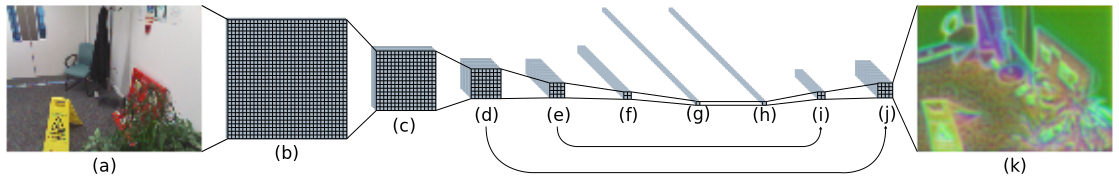
\includegraphics[width=\linewidth]{methodology/nn_architecture.png}
	\caption{Overview of the dense descriptor network. An input is presented at step (a). In each of sections (b-h), the network performs a max pooling operation to downsample the previous layer, followed by one to three convolution and nonlinearity (ReLU) operations. The number of filters is increased exponentially in each successive layer. Layers (i-k) each perform a deconvolution to create a dense descriptor at the original resolution. Additionally, layers (i) and (j) are summed with a convolution of earlier layers, transferring information from earlier in the network. During training, forward computation is performed on two input images, and the loss is computed using the final layer outputs from each image.}
	\label{fig:nn_architecture}
\end{figure}

\Fref{fig:nn_architecture} shows an outline of the network; we refer readers to the previous works for exact network dimensions and layouts. Notably, this network is fully convolutional (every layer is a convolution with shared parameters, or a pooling or nonlinearity operation). This is advantageous, as the network can be applied to images of any input dimensions (and the result is upsampled back to the same dimensions), and the parameter sharing allows for fewer total parameters and more efficient implementations than approaches with densely-connected layers.

Finally, we would like to select training data. In principle, for any pair of images, we could use pixels containing mutually observed points as positive training samples, and use every other pixel pair as negative samples. However, since there are quadratically many point pairs in the size of the image resolution, \cite{schmidt2017self} propose instead to sample up to 5000 positive point pairs (the images may contain fewer covisible points), and then 100 times as many negative point pairs. The loss of the negative point pairs then is divided by 100, to normalize for sample size.

We train our nets using a fork of the popular Caffe software \cite{jia2014caffe} provided by Schmidt \textit{et al}.. We find that the ADAM optimizer gives very fast convergence.

To demonstrate the idea behind this network, we use visualization technique suggested by original authors and train a descriptor with dimension $D=3$, so that we can visualize its components in RGB, as shown in \fref{fig:descriptor_3d}.

\begin{figure}[h]
	\centering
	\includegraphics[width=\linewidth]{methodology/descriptor_3d.png}
	\caption{A trained dense descriptor with descriptor size $D=3$. This shows an example from 7-Scenes.}
	\label{fig:descriptor_3d}
\end{figure}

%THIS DIDN'T REALLY WORK, MAYBE REMOVE THIS PARAGRAPH
%
%We also propose an alternative sampling scheme. In \cite{schmidt2017self}, almost every pixel contains an observation of a 3D mesh vertex. However, we have semi-dense depth data. As detailed in later sections, we only perform descriptor matching at non-empty locations in the depth map. Therefore, learning an embedding for points in image regions with low gradient is a waste of the feature space. Thus, we only keep negative descriptor pairs if both points have defined depth vales.

\section{Training a Visual Vocabulary}

After feature detection and descriptor computation, our images are now represented as a large ordered collection of high-dimensional ($D=128$ for SIFT and $D=32$ for learned features) features. We adopt the typical approach for image recognition, which is to represent the images instead as an unordered multiset (or bag) of quantized features (or visual words). In our circumstances, we have several million descriptors per training set, and we would like to quantize these to around $K=1000$ clusters.

Performing K-means clustering naively using Lloyd's algorithm \cite{lloyd1982least} on $N$ points requires $\mathcal{O}(N K D + K D) = \mathcal{O}(N K D)$ operations per update step, split between the assignment step and mean update step (see algorithm \ref{alg:lloyds}).

Instead, we follow the approximate K-means approach of Philbin \textit{et al}.\ \cite{philbin2007object}. This replaces the costly assignment step of Lloyd's algorithm by constructing a kd-tree of cluster centers and then performing searches on the tree for the closest cluster center to each datapoint (see algorithm \ref{alg:kdtreekmeans}). For a vanilla kd-tree, the results of this process are exactly equivalent to the naive method. However, this has an asymptotic runtime of $\mathcal{O}(K \log K + N D \log K + K D)$, which is a strict improvement for $N > K$. In practice, there is also a large constant time factor associated with maintaining the search tree, but we find it is not too significant.

Additionally, rather than performing exact lookups in the kd-tree, Philbin \textit{et al}. propose to speed up the search using an approximate-nearest-neighbors lookup scheme. We follow their approach by replacing the kd-tree in algorithm \ref{alg:kdtreekmeans} with an ensemble of fixed-depth trees \cite{muja2013flann}, resulting in even faster (but approximate) lookups.

\begin{algorithm}
	\caption{Lloyd's Algorithm}\label{alg:lloyds}
	\hspace*{\algorithmicindent} \textbf{Input} A set of $D$-dimensional points $\{x_1 \ldots x_N\}$ \\
	\hspace*{\algorithmicindent} \textbf{Output} A set of cluster centers $\{c_1 \ldots c_K\}$ minimizing $\sum_{i = 1}^N {\min_{j \in \{1 \dots K\}} ||x_i - c_j||_2^2}$
	\begin{algorithmic}[1]
		\Procedure{cluster}{}
		\State Initialize $\{c_1 \ldots c_K\}$ to be a random subset of $\{x_1 \ldots x_N\}$
		\While {not converged}
			\State let $\{S_1 \ldots S_K\}$ be a set of sets, initially all empty
			\Comment{Assignment}
			\For{i=1 to N}
				\State let $j^* \gets \argmin_{j \in \{1 \dots K\}} ||x_i - c_j||_2^2 $
				\State $S_{j^*} \gets S_{j^*} \cup \{i\}$
			\EndFor
			\For{j=1 to K}
			\Comment{Update}
				\State $c_j \gets \frac{\sum_{i \in S_j}{x_i}}{|S_j|}$
			\EndFor
		\EndWhile
		\EndProcedure
	\end{algorithmic}
\end{algorithm}

\begin{algorithm}
	\caption{kd-tree K-means}\label{alg:kdtreekmeans}
	\hspace*{\algorithmicindent} \textbf{Input} A set of $D$-dimensional points $\{x_1 \ldots x_N\}$ \\
	\hspace*{\algorithmicindent} \textbf{Output} A set of cluster centers $\{c_1 \ldots c_K\}$ minimizing $\sum_{i = 1}^N {\min_{j \in \{1 \dots K\}} ||x_i - c_j||_2^2}$
	\begin{algorithmic}[1]
		\Procedure{cluster}{}
		\State Initialize $\{c_1 \ldots c_K\}$ to be a random subset of $\{x_1 \ldots x_N\}$
		\While {not converged}
		\State construct a kd-tree \textit{t} from $\{c_1 \ldots c_K\}$
		\Comment{Tree Construction}
		\State let $\{S_1 \ldots S_K\}$ be a set of sets, initially all empty
		\Comment{Assignment}
		\For{i=1 to N}
		\State $j^* \gets$ \Call{NearestNeighborQuery}{\textit{t, $x_i$}}
		\State $S_{j^*} \gets S_{j^*} \cup \{i\}$
		\EndFor
		\For{j=1 to K}
		\Comment{Update}
		\State $c_j \gets \frac{\sum_{i \in S_j}{x_i}}{|S_j|}$
		\EndFor
		\EndWhile
		\EndProcedure
	\end{algorithmic}
\end{algorithm}

After training, each feature is assigned to its nearest cluster center, and therefore images are represented as a sparse vector of visual word frequencies.

\section{Building the Inverted Index}

A key advantage of representing images as histograms of visual words is ease of retrieval. The reason for this is simple: for a large enough visual vocabulary, the bag-of-words representation of a given image will be sparse, with relatively few non-zero visual word frequencies. In this representation, we compute image similarity between two images based solely on the overlap between their bags of words. Consequentially, to retrieve every image that has nonzero similarity to a query image, we only need to iterate over each query visual word and check images which contain that word. This is achieved using a map from visual words to sets of containing images (a so-called ``inverted'' index).

For this work, we use the DisLocation retrieval engine implementation of Sattler \textit{et al}.\ \cite{Sattler16CVPR}, which builds on earlier work \cite{Arandjelovic14a}. This is a two-tiered implementation based on hamming embeddings. It first performs inverted index retrieval, and then prunes matched features based on their hamming distance to the query feature under a randomized projection. This allows using fewer visual words (which encompass larger Voronoi cells), while achieving similar performance. In \cite{Sattler16CVPR}, the authors go onto compute a re-ranking based on geometric burstiness, although we disregard this feature.

\section{Pose Estimation}

\begin{figure}[h]
	\centering
	\def\svgwidth{0.8\columnwidth}
	\input{methodology/scale_ambiguity.pdf_tex}
	\caption{Two camera trajectories make an observation of the same scene from different viewpoints. However, because the two reconstructions are at a different scale, SE(3) pose alignment will work poorly.}
	\label{fig:scale_ambiguity}
\end{figure}

After retrieving an image from the training dataset, we would like relocalize the pose of the current test camera. As illustrated in \fref{fig:scale_ambiguity}, this is somewhat nuanced for the case of monocular vision due to the lack of an absolute scale. In prior works, such as \cite{shotton2013scene}, the authors seek a rigid transformation (6 degrees of freedom) to align 3D points, but this is only applicable because they have a known scale. In LSD-SLAM, the authors instead find a similarity transform (7 degrees of freedom) to align cameras. However, we care only to align single images to prior trajectories, and so finding a rigid transform expressed in the scale of a prior trajectory is sufficient for our work.

To this end, it would be convenient to use database images with associated depth maps, but only use a 2D pixel selection in the test query. This makes our task a problem of aligning 2D points in the query image to projections of 3D points from the database image. If we establish 2D-3D point correspondences between the test and train image, this becomes the perspective-n-point problem, with $n$ 2D-3D point correspondences.

First, to establish correspondences, we do descriptor matching. For our SIFT queries, we find nearest neighbor correspondences and then retain point pairs that pass the ratio test, as suggested in \cite{lowe1999object}. In other words, for a descriptor $m$ in the first image, we retrieve first nearest neighbor $n_1$ and second nearest neighbor $n_2$ descriptors in the second image. We only accept the correspondence $(m, n_1)$ if the following holds:

\begin{equation}
d(m, n_1) < r d(m, n_2)
\end{equation}

for the appropriate distance function $d$. Unless otherwise mentioned, we use $r=0.7$. This suggests that $(m, n_1)$ is salient compared to other possible correspondences. In the case of learned features, we simple require that each test feature corresponds to only one feature in the training image, as the distribution of features is not as spread out as in SIFT. Learning the correct distance function for such features is an open topic of research.

After finding feature correspondences, we compute a PnP solution. We use the formulation of \cite{lepetit2009epnp}, as implemented by \cite{opencv_library}, which requires 4 point correspondences in the minimal case. We repeat this in a RANSAC loop so as to reject spurious correspondences, and identify the solution with the maximum sized consensus set. We then perform iterative optimization using these inlier correspondences, again using the implementation of \cite{opencv_library}, which optimizes for a camera pose minimizing the camera plane projection error in the point correspondences.

\cleardoublepage
